\section{Module 4: Lecture 3\\Examples of Laplace and Z Transforms}


\subsection{Introduction}
In the previous lectures you were introduced to the definition of the \textit{Laplace transform} and the \textit{z transform}. In this lecture, we will look at a few examples of these transforms.\\
Also, throughout the subsequent lectures we will follow the convention that $x(t)$ has the Laplace transform $X(s)$, in the region of convergence $R_X$. And this relation is shown by
\[
x(t) \xrightarrow{\ \mathcal{L}\ } X(s)\ ,\ R_X
\]Similarly for the input $x[n]$ and its z-transform $X(z)$, in the region of convergence $R_X$, we write
\[
x[n] \xrightarrow{\ z\ } X(z)\ ,\ R_X
\]
\subsection{Laplace Transform Example}
Here, we will assume the input $x(t) = e^{2t}u(t) + e^{3t}u(t)$. We wish to find its \textit{Laplace transform} and the region of convergence.
\begin{align*}
	X(s) &= \int_{-\infty}^{\infty}{x(t)e^{-st}dt}\\
	 &= \int_{-\infty}^{\infty}{(e^{2t}u(t) + e^{3t}u(t))e^{-st}dt}\\
	 &= \int_{-\infty}^{\infty}{e^{2t}u(t)e^{-st}dt} + \int_{-\infty}^{\infty}{e^{3t}u(t)e^{-st}dt}\\
	 &= \int_{0}^{\infty}{e^{(2-s)t}dt} + \int_{0}^{\infty}{e^{(3-s)t}dt}
\end{align*}
Now the left term will converge only if $(2 - Re(s)) < 0$, i.e., $Re(s) > 2$. Similarly, the right term will converge only if $Re(s) > 3$. Hence the region of convergence is
\begin{align*}
	R_X &= (Re(s) > 2) \cap (Re(s) > 3) \\
	&= Re(s) > 3
\end{align*}

\begin{figure}[h!]
\begin{center}
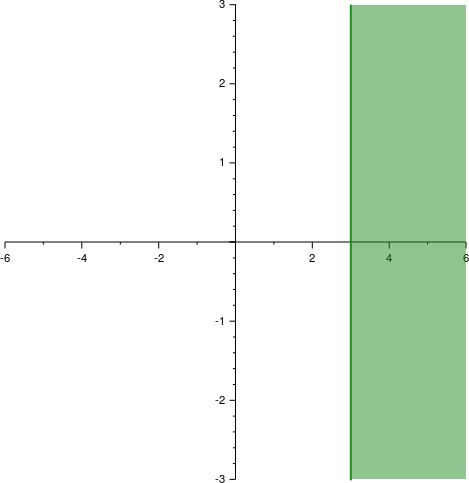
\includegraphics[width=5cm]{plot_1.png}
\end{center}
\caption{Region of convergence $R_X$ for the input  $x(t) = e^{2t}u(t) + e^{3t}u(t)$. (The green shaded region represents the ROC $Re(s) > 3$)}
\end{figure}

Continuing on the integral, 
\begin{align*}
	X(s) &= \frac{1}{(2 - s)}e^{(2-s)t}\Big|_0^{\infty} + \frac{1}{(3-s)}e^{(3-s)t}\Big|_0^{\infty}\\
	&= \frac{1}{(s - 2)} + \frac{1}{(s - 3)}
\end{align*}

\subsection{Z Transform Example}
Here, we will assume the input $x[n] = 2^{n}u[n] + 3^{n}u[n]$. We wish to find its \textit{z-transform} and the region of convergence.
\begin{align*}
X(z) &= \sum_{n=-\infty}^{\infty}{x[n]z^{-n}}\\
&= \sum_{n=-\infty}^{\infty}{(2^{n}u[n] + 3^{n}u[n])z^{-n}}\\
&= \sum_{n=-\infty}^{\infty}{2^{n}u[n]z^{-n}} + \sum_{n=-\infty}^{\infty}{3^{n}u[n]z^{-n}}\\
&= \sum_{n=0}^{\infty}{{(\frac{2}{z})}^{n}} + \sum_{n=0}^{\infty}{{(\frac{3}{z})}^{n}}
\end{align*}

Here, the left term only converges if $|\frac{2}{z}| < 1$, i.e., $|z| > 2$. Similarly from the right term, $|z| > 3$. 
Again, the region of converge
\[
	\mathbf{R_X : |z| > 3}
\]

\begin{figure}[h!]
\begin{center}
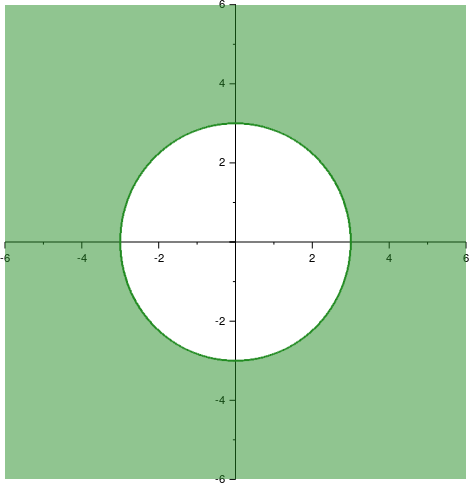
\includegraphics[width=5cm]{plot_2.png}
\end{center}
\caption{Region of convergence $R_X$ for the input  $x[n] = 2^{n}u[n] + 3^{n}u[n]$. (The green shaded region represents the ROC $|z| > 3$)}
\end{figure}

Continuing on the summation,
\[
	\mathbf{X(z) = \frac{z}{z-2} + \frac{z}{z-3}}
\]


\subsection{Conclusion}
In this lecture, we looked at a few examples of the \textit{Laplace transform} and the \textit{z-transform}. In the subsequent lectures, we will be looking at some properties of the \textit{Laplace transform} and the \textit{z-transform}, like linearity, modulation property, etc.







                



                     
